\documentclass{article}

\usepackage[english]{babel}
\usepackage[margin=3cm]{geometry}
\usepackage{graphicx}
\usepackage{float}
\usepackage{caption}
\usepackage{hyperref}
\usepackage{amsmath}
\usepackage{wrapfig}
\usepackage[parfill]{parskip}

% fonts
\usepackage[T1]{fontenc}
\usepackage{helvet}
\renewcommand{\familydefault}{\sfdefault}

\graphicspath{{img/}}

% theorem environment
\usepackage{amssymb}

\newtheorem{theorem}{Definition}[section]

\usepackage{enumitem}

\newenvironment{thmenum}
 {\begin{enumerate}[label=\upshape\bfseries(\roman*)]}
 {\end{enumerate}}


% code
\usepackage{minted}
\setminted{frame=single,framesep=3pt,linenos}
\usepackage{upquote}
\usepackage{color}

\begin{document}

\begin{titlepage}
    \author{Tuur Vanhoutte}
    \title{MLOps}
\end{titlepage}

\pagenumbering{gobble}
\maketitle
\newpage
\tableofcontents
\newpage

\pagenumbering{arabic}

\section{Introduction}

\begin{itemize}
    \item Deployment of deep learning models in an API
    \item Deploying services to Kubernetes with Docker
    \item Version Controlling with Git (to blame those who ruined the code)
    \item Automation pipelines to prepare data, train models and deploy applications
    \begin{itemize}
        \item Automated delivery (ready to deploy)
        \item Automated deployment (CI / CD)
    \end{itemize}
\end{itemize}

\subsection{Why do I need deployment automation}

\begin{itemize}
    \item Save time
    \item Increased accuracy
    \item Better documentation
    \item Autoscaling
\end{itemize}

\subsection{What will we do}

\begin{itemize}
    \item Object classification with a CNN
    \item Deployed with FastAPI 
    \item Scalable with Kubernetes
    \item Automated with CI/CD pipelines
    \begin{itemize}
        \item Yes, also automated AI Training!
    \end{itemize}
\end{itemize}


\subsection{The AI pipeline}

\begin{figure}[H]
    \centering
    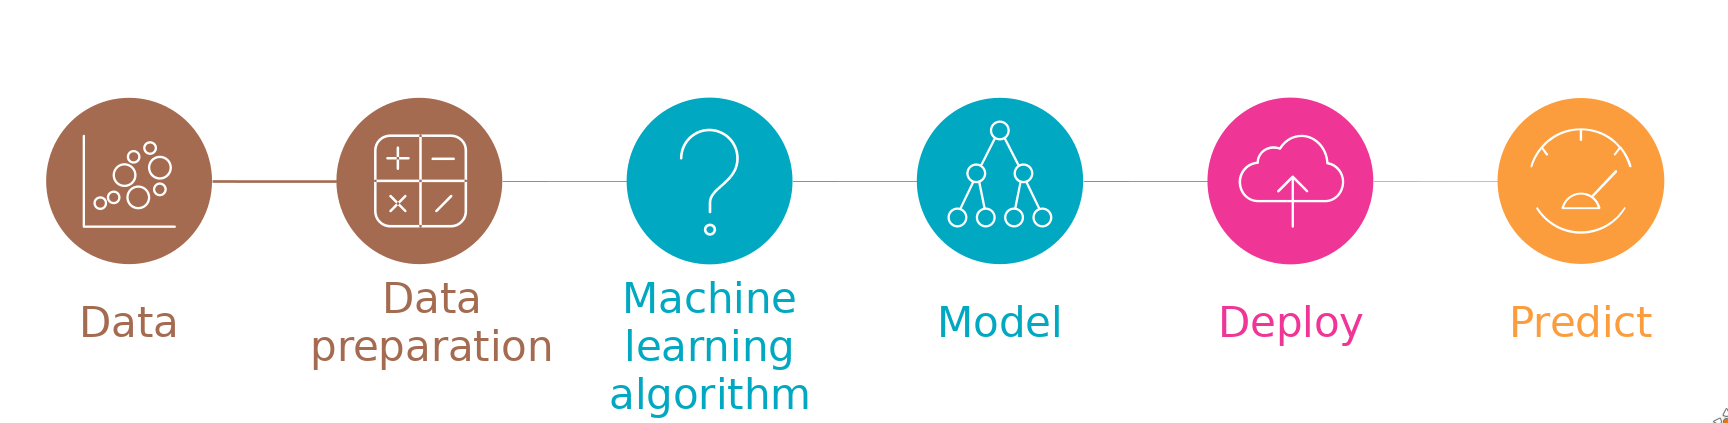
\includegraphics[width=0.8\textwidth]{complete-pipeline.png}
    \caption{The complete AI pipeline}
\end{figure}

\subsection{Teleport}

How to connect to your dedicated virtual machine? 
\textbf{Teleport} allows engineers and security professionals 
to unify access for SSH servers, Kubernetes clusters, 
web applications, and databases across all environments.

\subsubsection{Teleport Server Access}

\begin{itemize}
    \item One centralized login and user-management system
    \item Randomly generated passwords for your user account
    \item We manage all virtual machines your use can access
\end{itemize}

To \textbf{install and use Teleport}, see Leho.

\section{FastAPI}

TODO

\section{Docker}

TODO

\section{Kubernetes}

\subsection{What is Kubernetes?}

\begin{theorem}
    Kubernetes is a \textbf{portable}, \textbf{extensible}, \textbf{open-source} platform for \textbf{managing 
    containerized workloads and services}, that facilitates both \textbf{declarative configuration} and \textbf{automation}. 
    It has a large, rapidly growing ecosystem. Kubernetes services, support, and tools are widely available.
\end{theorem}

\begin{itemize}
    \item Service discovery and load balancing
    \item Storage orchestration
    \item Automated rollouts and rollbacks
    \item Self-healing
    \item Auto-scaling
\end{itemize}

\begin{figure}[H]
    \centering
    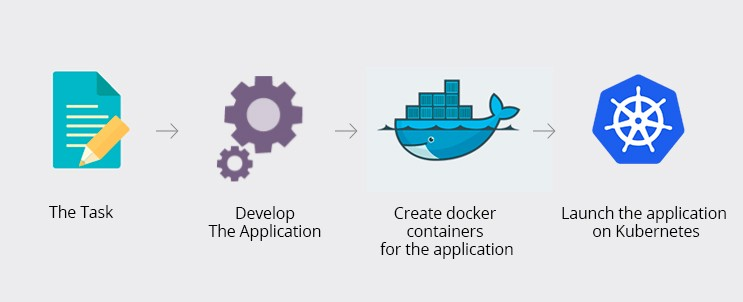
\includegraphics[width=0.5\textwidth]{img/kubernetes-workflow.jpg}
    \caption{Kubernetes workflow}
\end{figure}

\subsection{Architecture}

A Kubernetes cluster consists of a set of worker machines, called nodes, that run containerized applications. 
Worker nodes host the Pods that are the components of the application workload. 
The control plane manages the worker nodes and the Pods in the cluster. 
In production environments, the control plane usually runs across multiple computers and a cluster usually runs multiple nodes, 
providing fault-tolerance and high availability.

\begin{figure}[H]
    \centering
    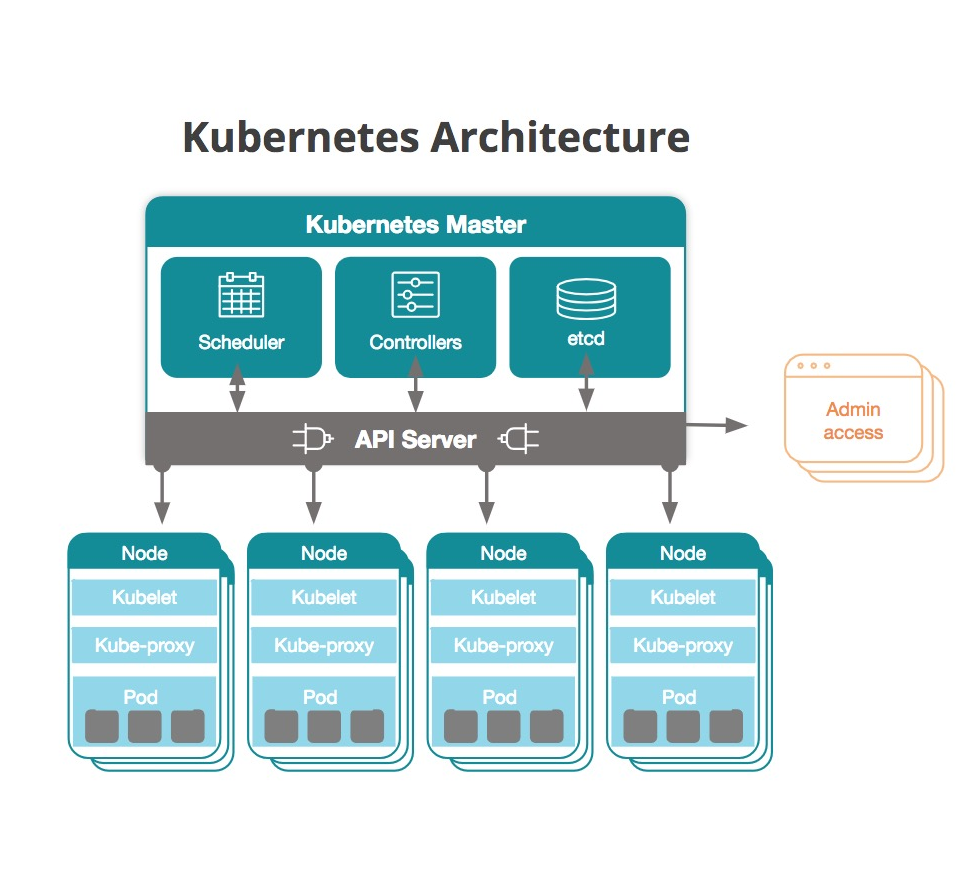
\includegraphics[width=0.5\textwidth]{img/kubernetes-architecture.png}
    \caption{Architecture}
\end{figure}

\subsubsection{Control Plane / Kubernetes Master}

\begin{itemize}
    \item Scheduler
    \begin{itemize}
        \item Makes sure that the number of desired pods is always running
        \item Keeps track of capacity and resources of nodes
        \item Assigns work to nodes based on availability
    \end{itemize}
    \item Controller
    \begin{itemize}
        \item responsible for registering nodes and monitoring health
    \end{itemize}
    \item etcd
    \begin{itemize}
        \item A persistent and distributed key-value data store
        \item Stores the state and configuration data for the entire cluster
    \end{itemize}
    \item API-server
    \begin{itemize}
        \item main access point to the control plane and master node
    \end{itemize}
\end{itemize}

\subsubsection{Node}

A node is a virtual machine. It has at least two tasks:

\begin{itemize}
    \item Kubelet
    \begin{itemize}
        \item Manages the state of a node
        \begin{itemize}
            \item Starting, stopping and maintaining application containers with instructions from the control plane
        \end{itemize}
        \item Collects performance and health information of node, pods and containers
        \begin{itemize}
            \item Shares those with the Control Plane
        \end{itemize}
    \end{itemize}
    \item Kube-proxy
    \begin{itemize}
        \item Network proxy
        \item Manages the Virtual IP addresses of pods and services
        \item Also works as a load balancer for services running on a node
    \end{itemize}
    \item Pod
\end{itemize}

\subsection{Objects}

Kubernetes objects are persistent entities in the Kubernetes system. 
Kubernetes uses these entities to represent the state of your cluster. Specifically, they can describe:

\begin{itemize}
    \item What containerized applications are running (and on which nodes)
    \item The resources available to those applications
    \item The policies around how those applications behave, such as restart policies, upgrades, and fault-tolerance
\end{itemize}

A Kubernetes object is a "record of intent"–once you create the object, 
the Kubernetes system will constantly work to ensure that object exists. 
By creating an object, you’re effectively telling the Kubernetes system what you want your cluster’s workload to look like; 
this is your cluster’s desired state.

\subsubsection{Building blocks}

\begin{itemize}
    \item \textbf{Pods}
    \item \textbf{Services} and EndPoints
    \item \textbf{Deployments}
    \item ReplicaSets
    \item DaemonSets
    \item StatefulSets
    \item \textbf{Ingress}
    \item PersistentVolumes and PersistentVolumeClaims
    \item ConfigMaps and Secrets
\end{itemize}

\subsubsection{Pods}

\begin{theorem}
    In Kubernetes, the \textbf{Pod} serves as a kind of basic, functional unit. 
    A pod is a set of containers, along with their shared volumes. 
\end{theorem}

As Kubernetes’ scheduler creates and deletes application pods unexpectedly, 
you should not rely on a particular pod. 
However, you do need to be able to access your application in a predictable manner. 
And to do that, Kubernetes provides the simplest form of load balancing traffic, namely a Service.

\subsubsection{Services}

\begin{theorem}
    A Kubernetes Service is an abstraction which defines a logical set 
    of Pods and a policy by which to access them - 
    sometimes called a micro-service. 
    The set of Pods targeted by a Service is (usually) determined by a Label Selector.
\end{theorem}

Services have IP addresses (used internally by Kubernetes) which are relatively stable. 
When a program element needs to make use of the functions abstracted by the service, 
it makes a request to the service, rather than an individual pod. 
The service then acts as a dispatcher, assigning a pod to handle the request. 
Thus, a client never connects to a container, but to a Pod, through a Service.

\subsubsection{Deployments and ReplicaSets}

\begin{theorem}
    A deployment is a YAML object that defines the pods and the number of container instances, called replicas, for each pod. 
    You define the number of replicas you want to have running in the cluster via a ReplicaSet.
\end{theorem}

\begin{theorem}
    A ReplicaSet is part of the deployment object. 
    So, for example, if a node running a pod dies, the replica set will ensure that another pod is scheduled on another available node.
\end{theorem}

\subsubsection{Daemonsets}

\begin{theorem}
    A DaemonSet ensures that all (or some) Nodes run a copy of a Pod. As nodes are added to the cluster, 
    Pods are added to them. As nodes are removed from the cluster, those Pods are garbage collected. 
    Deleting a DaemonSet will clean up the Pods it created.
\end{theorem}


Some typical uses of a DaemonSet are:

\begin{itemize}
    \item running a cluster storage daemon, such as glusterd, ceph, on each node.
    \item running a logs collection daemon on every node, such as fluentd or filebeat.
\end{itemize}

\subsubsection{StatefulSets}

\begin{theorem}
    Like a Deployment, a StatefulSet manages Pods that are based on an identical container spec. 
    Unlike a Deployment, a StatefulSet maintains a sticky identity for each of their Pods. 
    These pods are created from the same spec, but are not interchangeable: 
    each has a persistent identifier that it maintains across any rescheduling.

    If you want to use storage volumes to provide persistence for your workload, 
    you can use a StatefulSet as part of the solution. 
    Although individual Pods in a StatefulSet are susceptible to failure, 
    the persistent Pod identifiers make it easier to match existing volumes to the new Pods that replace any that have failed.
\end{theorem}


\subsubsection{PersistentVolumes and PersistentVolumeClaims}

PersistentVolumes

\begin{itemize}
    \item Define a storage volume in the cluster
    \item Independent lifecycle
    \item Otherwise: ephemeral data inside the pods
\end{itemize}

\subsubsection{ConfigMaps and Secrets}

\begin{itemize}
    \item Decouple configurations from hard-coded environment variables
    \item Separate Kubernetes object to share with Pods
    \item Difference: Secrets hold confidential information
    \item Example:
    \begin{itemize}
        \item Different configurations for Development, Staging and Production environments, quickly interchangeable
        \item Storing passwords and using it in your applications
    \end{itemize}
\end{itemize}

\subsection{Load balancer}

L4 Load Balancing (TCP)

\begin{itemize}
    \item Only available on Kubernetes Cloud Providers (GCP, AWS, Azure …)
\end{itemize}


L7 Load Balancing

\begin{itemize}
    \item Can redirect traffic to specific workloads based on request
    \item Ingress
\end{itemize}

\begin{figure}[H]
    \centering
    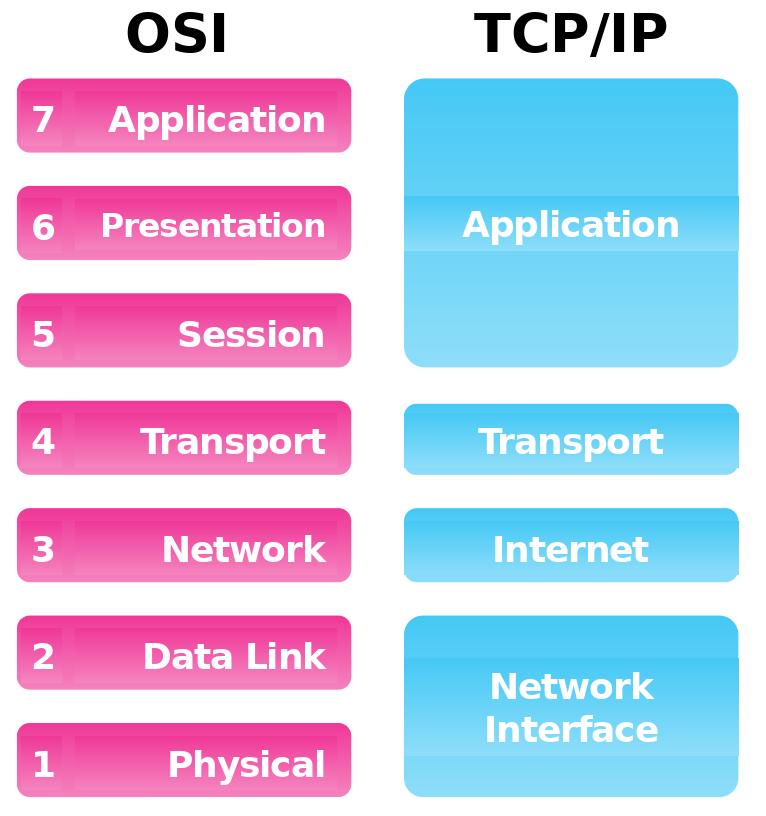
\includegraphics[width=0.4\textwidth]{img/osi-tcpip.png}
    \caption{Layers in OSI \& TCP/IP}
\end{figure}


\begin{itemize}
    \item Kube-proxy
    \begin{itemize}
        \item Load distribution
        \item Default: Randomly route to IP addresses based on iptables
        \item Previously: Round-robin 
    \end{itemize}
    \item Ingress
    \begin{itemize}
        \item Routes traffic based on request rules configured
        \item Deploy a Controller (like nginx)
        \item Deploy Resources
        \item Tip: Use Rancher to deploy Ingress Controllers and Resources (it has a UI for that)
    \end{itemize}
\end{itemize}


\subsection{Autoscaler}

Kubernetes uses the horizontal pod autoscaler (HPA) to monitor the resource demand and automatically scale the number of replicas. 
When changes in replica count are required, the number of replicas is increased or decreased accordingly.

You define the minimum and maximum number of replicas that can run. 
You also define the metric to monitor and base any scaling decisions on, such as CPU usage.

\begin{figure}[H]
    \centering
    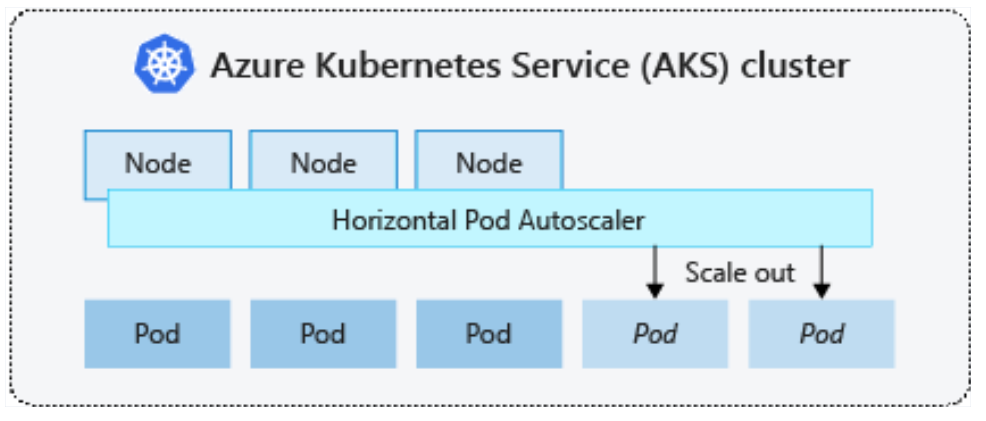
\includegraphics[width=0.5\textwidth]{img/autoscaler.png}
    \caption{Autoscaler}
\end{figure}

\subsection{YAML file}

\begin{minted}{yaml}
apiVersion: apps/v1
kind: Deployment
metadata:
  name: nginx-deployment
spec:
  selector:
    matchLabels:
      app: nginx
  replicas: 2 # tells deployment to run 2 pods
  template:
    metadata:
      labels:
        app: nginx
    spec:
      containers:
      - name: nginx
        image: nginx:1.14.2
        ports:
        - containerPort: 80
\end{minted}

\begin{itemize}
    \item apiVersion
    \begin{itemize}
        \item Which version of the Kubernetes API you’re using to create this object.
    \end{itemize}
    \item kind
    \begin{itemize}
        \item What kind of object you want to create
    \end{itemize}
    \item metadata
    \begin{itemize}
        \item Data that helps uniquely identify the object, including the name string, UID and optional namespace
    \end{itemize}
    \item spec
    \begin{itemize}
        \item What state you desire for the object
    \end{itemize}
\end{itemize}


\subsection{Helm}


\begin{theorem}
    Helm is an application package management registry for Kubernetes, maintained by the CNCF. 
    Helm "charts" are pre-configured software application resources you can download and deploy and in your Kubernetes environment.
\end{theorem}

According to a 2018 CNCF survey, 68\% of respondents said Helm was the preferred package management tool for Kubernetes applications. 
Helm charts can help DevOps teams come up to speed more quickly with managing applications in Kubernetes; 
it allows them leverage existing charts that they can share, version, and deploy into their dev and production environments.

\begin{itemize}
    \item Package manager
    \item We can create custom Helm charts
\end{itemize}

\begin{minted}{yaml}
    spec:
      containers:
      - args:
        - uwsgi
        - --ini
        - app.ini
        env:
        {{- range $key, $value := .Values.env.webapp }}
        - name: {{ $key }}
          value: {{ $value | quote }}
        {{- end }}
        image:{{ .Values.repository }}
        /basicwebapp:{{ .Values.app.version.webapp }}
        name: {{ $name }}
        resources: {}
      restartPolicy: Always
\end{minted}

\begin{itemize}
    \item Organised in template.yaml files
    \item Placeholders inside yaml files
    \item Values.yaml to fill placeholders
    \item Installing and upgrading versions of a release through CLI
    \item Loops, conditionals, variables, filters, values and more …
\end{itemize}

\section{Rancher}

\begin{theorem}
    Rancher is a complete software stack for teams adopting containers. 

    It addresses the operational and security challenges of managing multiple Kubernetes clusters, 
    while providing DevOps teams with integrated tools for running containerized workloads.
\end{theorem}

\begin{itemize}
    \item Simple, intuitive UI to get started with Kubernetes
    \item Multi-cloud and hybrid-cloud Kubernetes solutions
    \item Fast way to set up on-premises Kubernetes clusters
    \item Includes CI/CD pipelines for DevOps operations
\end{itemize}

\begin{figure}[H]
    \centering
    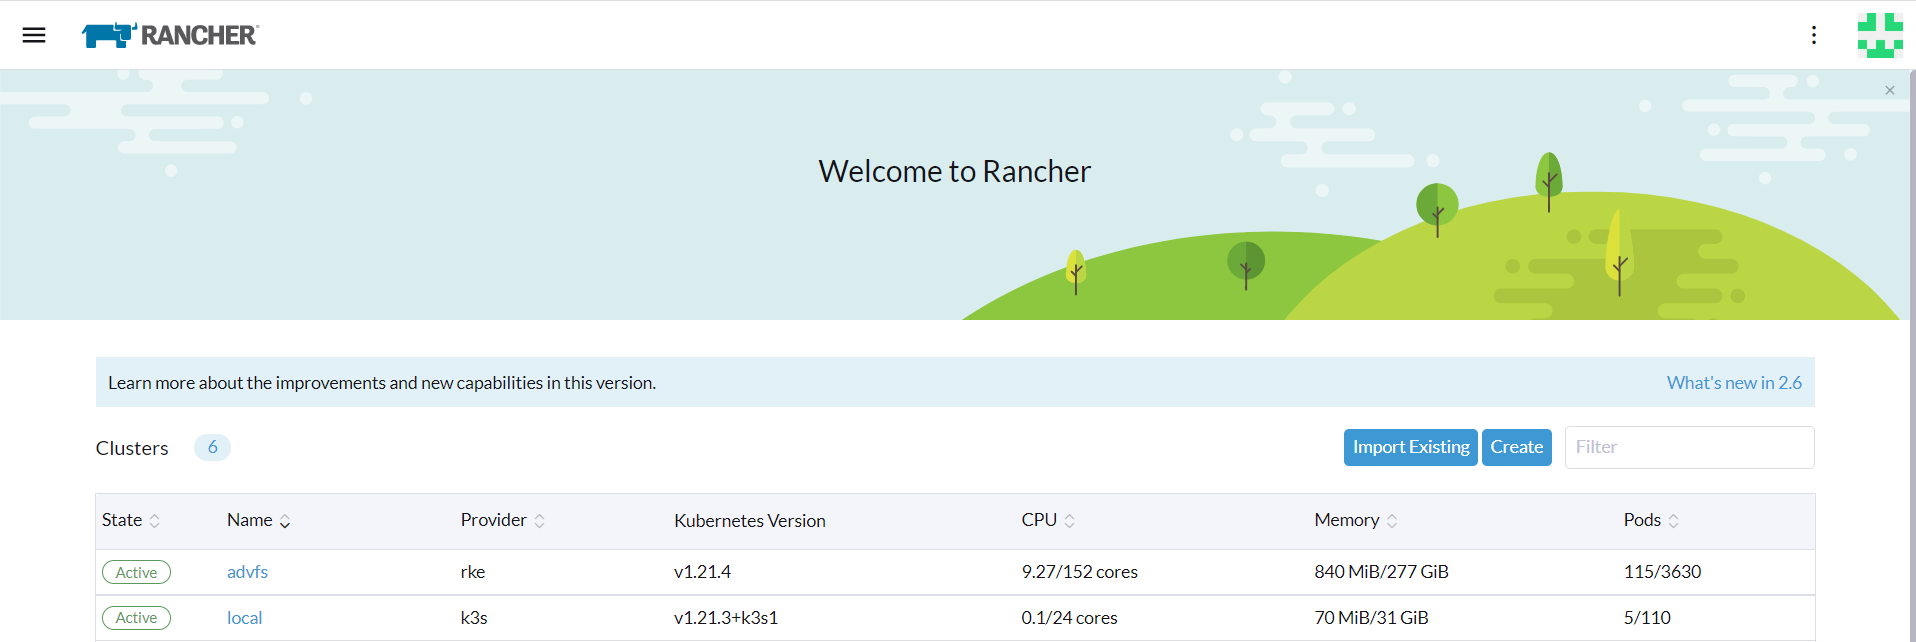
\includegraphics[width=0.75\textwidth]{img/rancher.png}
    \caption{Rancher welcome page}
\end{figure}

\begin{figure}[H]
    \centering
    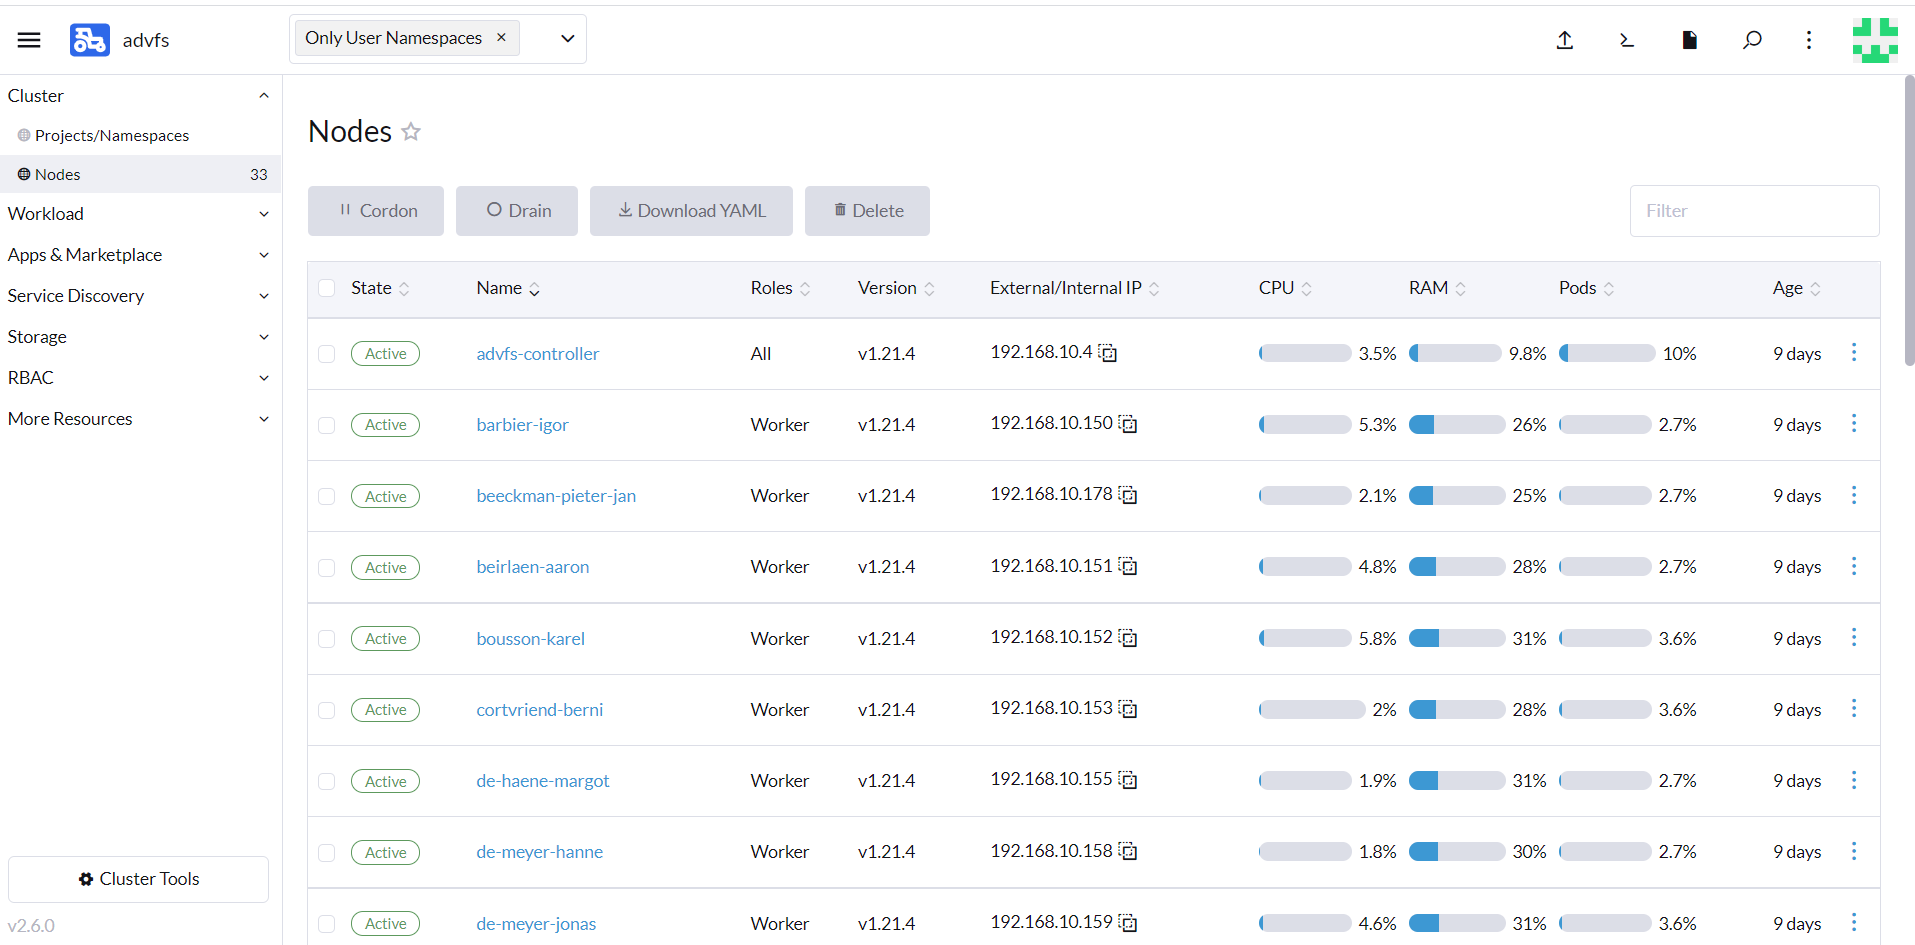
\includegraphics[width=0.75\textwidth]{img/rancher2.png}
    \caption{List of nodes}
\end{figure}

\begin{figure}[H]
    \centering
    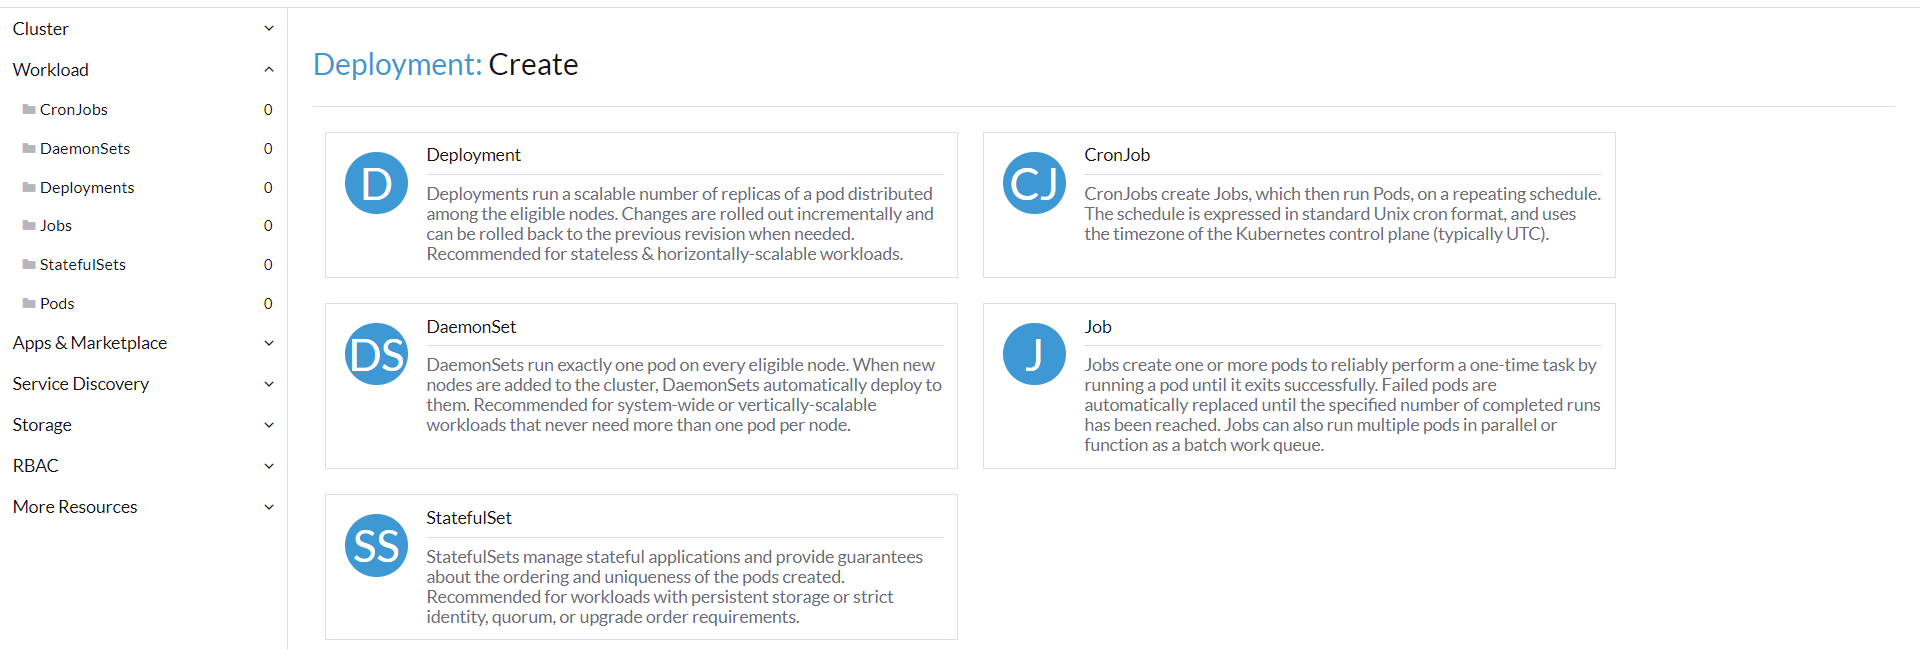
\includegraphics[width=0.75\textwidth]{img/rancher3.png}
    \caption{Deployment}
\end{figure}

\begin{figure}[H]
    \centering
    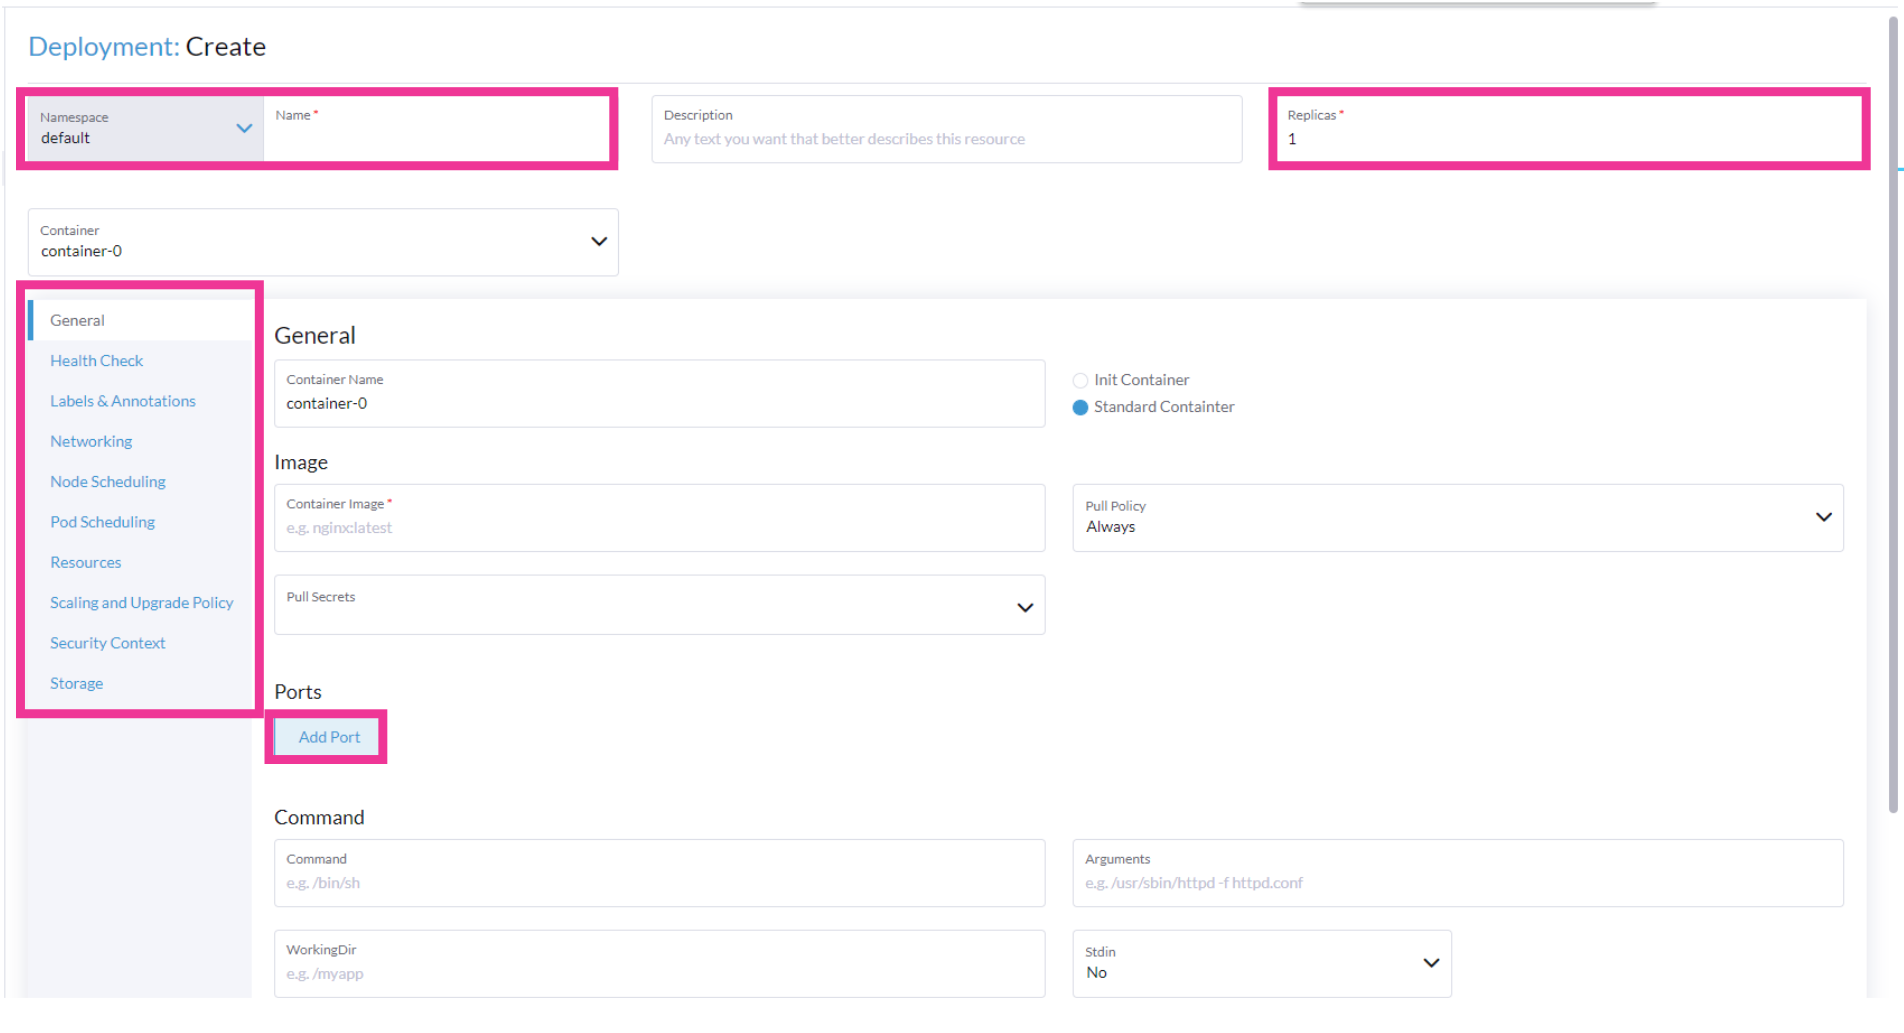
\includegraphics[width=0.75\textwidth]{img/rancher4.png}
    \caption{Creating a Deployment}
\end{figure}

\begin{figure}[H]
    \centering
    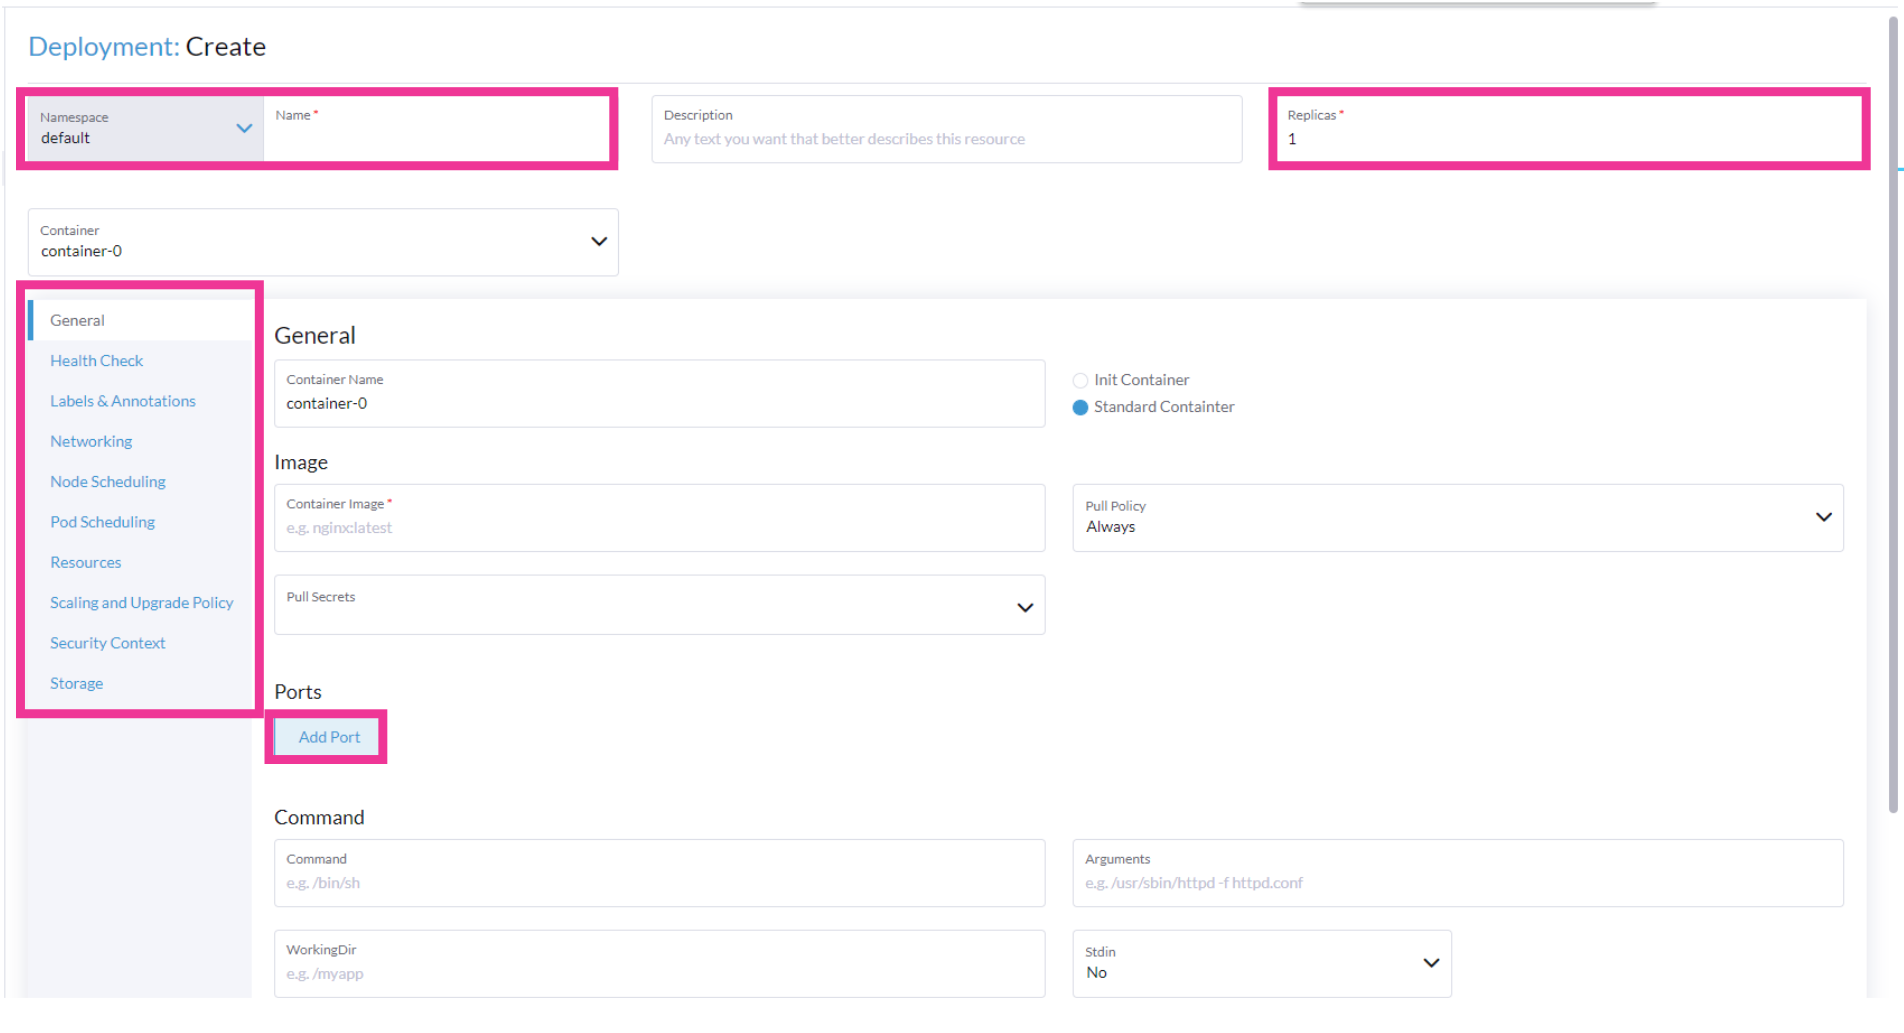
\includegraphics[width=0.75\textwidth]{img/rancher4.png}
    \caption{Creating a Deployment}
\end{figure}


\subsection{What we learned}

\begin{itemize}
    \item Why Kubernetes is useful for microservices
    \item The Kubernetes Building Blocks
    \item How autoscaling in Kubernetes works
    \item Different kinds of Load Balancing options
    \item How to write a YAML file for a Kubernetes object
    \item What the advantages of Helm charts are
    \item What Rancher does for us
\end{itemize}

Setting up Rancher and Kubernetes: see labs

\end{document}